\documentclass[../main.tex]{subfiles}
\begin{document}
	\begin{defin}
		\underline{Кв. ф называется:}
		\begin{mylist}
			\item \underline{Положительно (отрицательно) определенной}, если $\forall x \neq 0 \; \; \; \underset{(<0)}{f(x) > 0} \Leftrightarrow \underset{(f<0)}{f>0}$
			\item \underline{Положительно (отрицательно) полуопределенной}, если $\forall x \neq 0 \; \; \; \underset{(\leq 0)}{f(x) \geq 0} \Leftrightarrow \underset{(f\leq 0)}{f \geq 0}$
			\item \underline{Неопределенной}, если $\exists x: f(x) > 0 \Space \exists y: f(y) < 0 \Leftrightarrow f <> 0$
		\end{mylist}
	\end{defin}
	\begin{remark}
		\begin{mylist}\
			\item Сравним с оператором $\A > 0$ и т.п.
			\item $f> 0 \Leftrightarrow \forall x: f(x) \geq 0$, причем $f(x) = 0 \Leftrightarrow x = 0$ и т.д.\n
			$f \geq 0 \Leftrightarrow \forall x: f(x) \geq 0$ и $\exists x \neq \0: f(x) > 0$ и т.д.
		\end{mylist}
	\end{remark}
	\textbf{Критерий знакоопределенности кв. ф.}\n
	$\underset{(f<0)}{f>0} \Leftrightarrow \underset{(<0)}{A>0} \Leftrightarrow$ все с.ч. $\underset{(\lambda < 0)}{\lambda > 0} \Leftrightarrow \begin{array}{l}
		\sigma(f) = (n, 0, 0) \Space \text{(невырожд. } rg f = n = \sigma^+)\n 
		(\sigma(f) = (0, n, 0) \Space (rg f = n = \sigma^-))
	\end{array} \n 
	\underset{(\lambda \leq 0)}{\lambda \geq 0} \Leftrightarrow \begin{array}{l}
	\sigma(f) = (k\neq 0, 0, m\neq 0) \Space \text{(вырожд. } rg f = \sigma^+ = k < n \Space k+m = n)\n 
	(\sigma(f) = (0, k\neq 0, \neq 0) \Space (rg f = k = \sigma^- < n \Space k+m = n))
	\end{array} \n 
	f <> 0 \Leftrightarrow A <> 0 \Leftrightarrow \begin{array}{l}
		\exists \text{ с.ч. } \lambda> 0\\
		\exists \text{ с.ч. } \mu < 0
	\end{array} \Leftrightarrow \sigma(f) = (k \neq 0, m \neq 0, l)$
	\begin{examples}
		\begin{mylist}\
			\item $f(x) = 3x_1^2 - 2x_2^2 + x_3^2 \n 
			\sigma(f) = (2, 1, 0) \Space \R^3 \n 
			\sigma(f) = (2, 1, n-3) \Space \R^n \; \; \; n > 3 \n 
			f \neq 0\Space  \begin{matrix}
				x_2 = 0 \; \; \; x_1 = x_3 = 1&:& f(x) = 4 > 0 \\
				x_1 = x_3 = 0 \; \; \; x_2 = 1&:& f(x) = -2 < 0
			\end{matrix}$\ \\
			\item $f(x) = 3x_1^2 + 2x_2^2 + x_3^2 + 0 \cdot x_4^2\n 
			\sigma(f) = (3, 0, n-3) \Space \R^n \n 
			\begin{matrix}
				n = 3 & f > 0\\
				n > 3 & f \geq 0
			\end{matrix} \Sspace \begin{matrix}
				x_1 = x_2 = x_3 = 0 \\
				x_4 = 1 \Space x \neq \0 \\ 
				f(x) = 0 \Rightarrow f \geq 0
			\end{matrix}$
		\end{mylist}
	\end{examples}
	\begin{theorem}[Критерий Сильвестра]\ \\
		$\triangle_k \neq 0 \; \; \; k = 1 \ldots n \Rightarrow  \Sspace \Sspace \triangle_k = det A_k\n 
		f> 0 \Leftrightarrow \triangle_1 > 0 \; \; \; \triangle_2 > 0 \; \; \; \triangle_3 > 0 \; \; \; \ldots \triangle_n > 0 \n 
		f<0 \Leftrightarrow \triangle_1 < 0 \; \; \; \triangle_2 > 0 \; \; \; \triangle_3 < 0 \; \; \; \ldots (-1)^n \triangle_n > 0$
	\end{theorem}
	\begin{proof}
		Метод Якоби: $x = Q y \Space Q$ унитреуг. \Space $f(x) = x^T A x \n 
		f(x) = \triangle_1 y_1^2 + \frac{\triangle_2}{\triangle_1} y_2^2 + \ldots
		 + \frac{\triangle_n}{\triangle_{n-1}} y_n^2\n 
		 f>0 \Leftrightarrow \triangle_1 > 0 \; \; \; \frac{\triangle_2}{\triangle_1} > 0 \; \; \; \ldots
		  \frac{\triangle_n}{\triangle_{n-1}} > 0\; \; \;  \Leftrightarrow \; \; \; \triangle_k > 0 \; \; \; \forall k = 1 \ldots n$\n 
		  $f < 0 \Leftrightarrow \triangle_1 < 0 \; \; \; \frac{ \triangle_2}{\triangle_1} < 0 \; \; \; \ldots
		   \frac{\triangle_n}{\triangle_{n-1}} \; \; \; \Leftrightarrow \; \; \; \triangle_1 < 0 \; \; \; \triangle_2 > 0 \; \; \; \triangle_3 < 0 \ldots$
	\end{proof}
	\begin{corollary}
		$\triangle_k \neq 0 \; \; \; k = 1 \ldots n-1\n 
		f \geq 0 \; \; \; \Leftrightarrow \; \; \; \triangle_1 > 0 \; \; \; \ldots \triangle_{n-1} > 0 \; \; \; \triangle_n = 0 \Space$ ($f \leq 0$ аналогично)
	\end{corollary}
	\begin{examples}
		\ \\
		$A = \begin{pmatrix}
			0 & 1 & -1 \\
			1 & 2 & 1\\
			-1 & 1 & 3
		\end{pmatrix} \Space
		 \triangle_1 = 0 \Rightarrow$ нельзя применять критерий Сильвестра\n 
		 $f(x) = x^T A x \n 
		 \begin{matrix}
		 x_1 \rightarrow y_2 \n 
		 x_2 \rightarrow y_1 \n 
		 x_3 \rightarrow y_3
		 \end{matrix} \leadsto g(y) = y^T B y \Space B = \begin{pmatrix}
			 2 & 1 & 1 \\
			 1 & 0 & -1 \\
			 1 & -1 & 3
		 \end{pmatrix}\n 
		 x = Q y \Space \underset{\text{невыр}}{Q} = \begin{pmatrix}
			 0 & 1 & 0\\
			 1 & 0 & 0\\
			 0 & 0 & 1
		 \end{pmatrix}
		 $
	\end{examples}
	\begin{remark}
		$\boxed{f> 0 \Leftrightarrow - f < 0}$ \Sspace $det \begin{pmatrix}
			- a_{11} & \ldots & - a_{1n} \\
			\ldots\\
			- a_{n1} & \ldots & - a_{nn}
		\end{pmatrix} = (-1)^n det A\n 
		- (\lambda_1 y_1^2 + \ldots + \lambda_n y_n^2) = - \lambda_1 y_1^2 - \ldots - \lambda_n y_n^2$
	\end{remark}
	\textbf{Применение в исследовании экстремумов}\n 
	$f(\overset{=P}{x, y}) = f(\overset{=P_0}{x_0, y_0}) + \underset{\text{необходимое условие экстр.}}{\cancel{\frac{df}{1!}(P_0)}} + \frac{d^2 f}{2!}(P_0) + \mathscr{o} (\sqrt{\triangle x^2 + \triangle y^2}^2)\n 
	P_0$ -- $(.)$ экстремума\n 
	$\pu P_0 \; min \Space \underbracket{f(P) - f(P_0)}_{>0} = \frac{1}{2} (\underbracket{f''_{xx}(P_0) dx^2 + 2 f''_{xy}(P_0)dxdy + f''_{yy}(P_0) dy^2}_{>0}) + \mathscr{o}(\ldots)\n$
	$\overset{\nearrow}{\text{Кв. ф. от }}$$\triangle x, \triangle y$ \Space $\begin{matrix}
		\begin{matrix}
			dx = \triangle x\\
			dy = \triangle y
		\end{matrix}\n 
		\triangle P = \begin{pmatrix}
			\triangle x \\
			\triangle y
		\end{pmatrix}
	\end{matrix}\n 
	\downarrow$ матрица \n 
	$A = \begin{pmatrix}
		f''_{xx} & f''_{xy}\\
		f''_{xy} & f''_{yy}
	\end{pmatrix} \Space$ кв. ф. $(\triangle P)^T A (\triangle P)$\n 
	Критерий Сильвестра: кв. ф. = $d^2 f > 0 \Leftrightarrow f''_{xx} (P_0) > 0, f''_{xx} f''_{yy} - (f''_{xy})^2 > 0$ достаточное усл-е для min \n 
	\slide{190px} $<0 \Leftrightarrow f''_{xx}(P_0) < 0, f''_{xx} f''_{yy} - (f''_{xy})^2 < 0$ достат. усл-е max\n 
	$\underset{\text{нет экстр}}{f \neq 0} \Space f''_{xx} f''_{yy} - (f''_{xy})^2 < 0 \n $
	И такой еще есть случай: $
	\begin{pmatrix}
		0 & 2 \\ 2 & 0
	\end{pmatrix} \Space \begin{pmatrix}
		- \lambda & 2 \\ 2 & - \lambda
	\end{pmatrix} \Space \lambda^2 - 4 = 0 \Rightarrow \lambda = \pm 2 \Rightarrow f \neq 0$
	\subsection{Некоторые задачи из теории кв. форм}
	\textbf{Задача 1:} $\Space f, g \Space f \overset{Q?}{\leadsto} g \n 
	\begin{matrix}f(x) = x^T A x\\
	g(y) = y^T B y\end{matrix} \Space \exists \underset{\text{невыр.}}{Q?} \Space A = Q^T B Q$\n 
	"Да" $\Leftrightarrow \sigma(f) = \sigma(g) \n 
	\boxed{x = Q_1 Q_2^{-1} y} \Space \boxed{Q = Q_1 Q_2 ^{-1}}\n 
	f(x) \rightarrow g(y) \Space \downarrow y = Q_2 z \Space \uparrow z = Q^{-1}_2 y \n 
	f(x) \rightarrow$ нормальн. вид $t(z)$ т.к. $\sigma (f) = \sigma(g)$\n 
	\textbf{Задача 2:} $\Space f(x), g(x) \overset{Q?}{\leadsto}$ канонич.\n 
	"Не всегда $\exists Q$"\n 
	\underline{Пример:} \Space $f(x) = x_1^2 \Space g(x) = x_1 x_2 \Space \R^2 \n 
	\pu \exists
	 Q = \begin{pmatrix}
		 q_{11} & q_{12}\\
		 q_{21} & q_{22}
	 \end{pmatrix}$ т.ч. $f, g \rightarrow$ канонич. \n 
	 $x = Q y \Space f(x) = (q_{11} y_1 + q_{12} y_2)^2 \Rightarrow q_{11} q_{12} = 0 \Rightarrow \pu q_{12} = 0$ т.к. $Q$ невыр. $q_{11} \neq 0 \Rightarrow\n 
	 \Rightarrow g(x) = q_{11} y_1 \cdot (q_{21} y_1 + q_{22} y_2) \Rightarrow q_{11}\cdot q_{22} = 0 \Rightarrow q_{22} = 0 \Rightarrow Q$ вырожд. $\Rightarrow$ невозможно.\n 
	 $\boxed{\pu \dunderline{f > 0}} \Rightarrow ``\exists Q`` \n 
		 f > 0 \Space \underset{\text{f к норм. виду}}{\rightarrow} x = Q_1 y \Space \tilde{f}(y) = y_1^2 + y_2^2 + \ldots + y_n^2 \Space y = \overset{\text{ортогон. преобр.}}{Q_2 z} \Space \tilde{\tilde{f}}(z) = z_1^2 + \ldots + z_n^2 \n 
		 g \Sspace \tilde{g} (y) \Sspace \Sspace \tilde{g} \text{ к канон. виду } \rightarrow \tilde{\tilde{g}}(z) \text{ канон.}\n$
	$\tilde{f} \leftrightarrow E \n 
	\tilde{\tilde{f}} \leftrightarrow
	 Q_2^T E Q_2 = \overset{= Q^{-1}_2}{Q_2^T} \underset{\stackrel{\uparrow}{\text{ортог.}}}{Q_2} = E$
	 \subsection{Приведение поверхности второго порядка к каноническому виду}
	 $V_3 (x, y, z) \leftrightarrow \R^3 \n 
	 \underbracket{a_{11} x^2 + a_{22} y^2 + a_{33} z^2 + 2 a_{12} xy + 2 a_{13} x z + 2 a_{23} y z}_\mathlarger{\text{квадрат. форма } f (x, y, z) = v^T A v} + 2 a_1 x + 2 a_2 y + 2 a_3 z + a_0 = 0$\n 
	 $v = \begin{pmatrix}
		 x\\y\\z
	 \end{pmatrix}\n 
	 v^T A v + 2 a^T v + a_0 = 0 \Space a = \begin{pmatrix}
		 a_1\\a_2\\a_3
	 \end{pmatrix} \Space A = \begin{pmatrix}
		 a_{11} & a_{12} & a_{13}\\
		 a_{12} & a_{22} & a_{23}\\
		 a_{13} & a_{23} & a_{33}
	 \end{pmatrix} \Space A = A^T$\n 
	 $f(v) = 2(a, v) + a_0 = 0$\n 
	 Осуществим поворот. \\
	 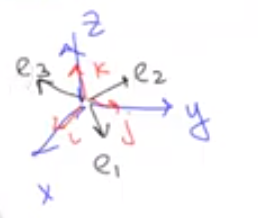
\includegraphics[width=100px]{pic34}\n
	 $T_{\underset{\text{о.н.б.}}{(ijk)} \rightarrow \underset{\text{о.н.б.}}{e_1 e_2 e_3}} = Q_{\text{ортог.}}$, т.ч. $f(v) \leadsto$ канонич. вид\n
	 $e_1, e_2, e_3$ -- с.в. $A$ попарно-ортог. и норм.\Sspace \underline{пр. тройка} $\Leftrightarrow det(e_1 e_2 e_3) = 1$\n 
	 $\begin{matrix}
		 \begin{pmatrix}
			 x\\y\\z
		 \end{pmatrix}\\v
	 \end{matrix} = \overset{\stackrel{Q}{||}}{T} \begin{matrix}
		 \begin{pmatrix}
			 x'\\y'\\z'
		 \end{pmatrix}\\v'
	 \end{matrix} = Q \begin{pmatrix}
		 x'\\y'\\z'
	 \end{pmatrix} \n 
	 f(v) + 2(a, v) + a_0 = \lambda_1 x'^2 + \lambda_2 y'^2 + \lambda_3 z'^2 + \boxed{2 a^T (Q} v') + a_0 = 0 \n 
	 \lambda_i$ с.ч. $A$\n 
	 $\boxed{\lambda_1 x'^2 + \lambda_2 y'^2 + \lambda_3 z'^2 + 2 a'_1 x' + 2 a'_2 y' + 2a_3 ' z' + a_0 = 0}$\n 
	 \textbf{I. $\lambda_1 \neq 0 \; \; \; \lambda_2 \neq 0 \; \; \; \lambda_3 \neq 0$}\n 
	 Если $a'_i \neq 0 $ выделяем полные квадраты по этой переменной \n 
	 $\lambda_1 x'^2 + 2 a'_1 x' = \lambda_1 (\underbracket{x'^2 + 2 \frac{a'_1}{\lambda_1} x' + \frac{a_1'^2}{\lambda_1^2}}_{(x' + \frac{a'_1}{\lambda_1})^2})- \frac{a_1'^2}{\lambda_1}\n 
	 \left[\begin{array}{ccl}
	 	x'' &=& x' + \frac{a'_1}{\lambda_1}\n 
	 	y'' &=& y' + \frac{a'_2}{\lambda_2}\n 
	 	z'' &=& z' + \frac{a'_3}{\lambda_3}
	 \end{array}\right.$ Параллельный перенос с.к. $O x' y' z' \leadsto O '' x''y''z''\n 
	 O'' = (-\frac{a'_1}{\lambda_1}, -\frac{a'_2}{\lambda_2}, - \frac{a'_3}{\lambda_3})$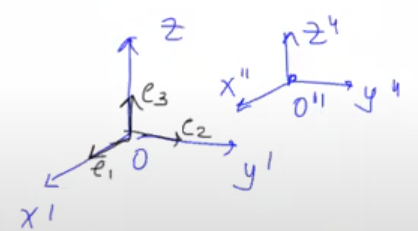
\includegraphics[width=170px]{pic35}\n 
	 $\boxed{\lambda_1 x''^2 + \lambda_2 y''^2 + \lambda_3 z''^2 + a'_0 = 0}$\n
	 \underline{a$'_0 \neq 0$}\n 
	 $\rightarrow \alpha x''^2 + \beta y''^2 + \gamma z''^2 = 1 \n 
	 \alpha, \beta, \gamma > 0$ Эллипсоид \n 
	 $\alpha, \beta > 0, \gamma < 0$ однополостной гипербол.\n 
	 $\alpha, \beta < 0, \gamma > 0$ двуполостной гиперболоид \n 
	 $\alpha, \beta, \gamma < 0$ --- $\emptyset$\n
	 \underline{$a'_0 = 0$}\n 
	 $\alpha x''^2 + \beta y''^2 = z''^2 \n 
	 \alpha, \beta > 0\\
	 \alpha \cdot \beta < 0$ --- конус\n
	 $\alpha, \beta < 0 \; \; \; x'' = y'' = z'' = 0$ --- точка\n
	 \textbf{II. $\lambda_1 \neq 0 \; \; \; \lambda_2 \neq 0 \; \; \; \lambda_3 = 0$}\n 
	 Аналогично $I$ выделяем полные квадраты для $\lambda_1, \lambda_2 \leadsto$ параллельный перенос \n если $a_3 \neq 0 \leadsto$ парал. перенос\n 
	 $
	 \left[\begin{array}{ccl}
	 	x'' &=& x' + \frac{a'_1}{\lambda_1}\\
	 	y'' &=& y' + \frac{a'_2}{\lambda_2}\\
	 	z'' &=& z' + \frac{a'_0}{2 a_3}
	 \end{array}\right. \underset{\text{парал. перенос}}{\leadsto} O x' y' z' \leadsto O'' x'' y'' z''\n 
	 O'' = (- \frac{a'_1}{\lambda_1}, - \frac{a_2'}{\lambda_2}, - \frac{a_3'}{2a_3})$\n
	\begin{mylist}
		\item $a'_3 \neq 0 \Space \begin{matrix}
			\boxed{\lambda_1 x''^2 + \lambda_2 y''^2 + 2 a'_3 z'' = 0}\n 
			\alpha x''^2 + \beta y''^2 = z''
		\end{matrix} \Space \begin{matrix}
			\alpha \cdot \beta > 0 \Space \text{\underline{Эллиптич. парабол.}}\\
			\alpha \cdot \beta < 0 \Space \text{\underline{Гипербол. парабол.}}
		\end{matrix}$
		\item $a'_3 = 0, \; \; z'' = z' \Space \boxed{\lambda_1 x''^2 + \lambda_2 y''^2 + a'_0 = 0}\n 
		\underline{a'_0 \neq 0}\n 
		\alpha x''^2 + \beta y''^2 = 1 \Space \begin{matrix}
			\alpha, \beta > 0 \text{ -- эллимптич. цилиндр}\\
			\alpha \cdot \beta < 0 \text{ -- гиперб. цилиндр}\\
			\alpha, \beta < 0 {\text{ -- }} \emptyset 
		\end{matrix}\n 
		\underline{a' = 0}\n 
		\alpha x''^2 = y''^2 \Space \begin{matrix}
			\alpha > 0 \Space y'' = \pm \sqrt \alpha x'' \text{ -- пара пересек. пл-тей}\\
			\alpha < 0 \Space x'' = y'' = 0 \text{ -- прямая, вдоль оси z''}
		\end{matrix}$
	\end{mylist}
	\textbf{III. $\lambda_1 \neq 0 \; \; \; \lambda_2 = \lambda_3 = 0$}\n 
	$\boxed{\lambda_1 x''^2 + 2 a_2' y' + 2 a'_3 z' + a_0 ' = 0} \Space x'' = x' + \frac{a'_1}{\lambda_1}$ паралл. перенос\n
	\begin{mylist} 
		\item $a'_2 \neq 0 \; \; \; a'_3 \neq 0 $ поворот в плоскости $O'' y' z'$ чтобы убрать слагаемое с переменной $z$\n 
		$\left[\begin{array}{ccl}
			y' &=& \cos \phi y'' - \sin \phi z''\\
			z' &=& \sin \phi y '' + \cos \phi z ''
		\end{array}\right. \Rightarrow \n 
		\Rightarrow 2 a'_2 (\cos \phi y'' - \sin \phi z'') + 2 a'_3 ( \sin \phi y '' + \cos \phi z'') = y'' (\underbracket{\ldots}_{a''/2}) + z'' (\underbracket{- 2 a'_2 sin \phi + 2 a'_3 \cos \phi}_{=0}) \n 
		\tan \phi = \frac{a'_3}{a'_2}\n 
		\leadsto \boxed{\lambda_1 x''^2 + 2 a''_2 y'' + a'_0 = 0}$ парабол. цилиндр
		\item $a'_2 \neq 0 \Space a'_3 = 0 $ попадает сразу в конец первого случая
		\item $a'_2 = a'_3 = 0 \Space \boxed{\lambda_1 x''^2 + a'_0 = 0} \rightarrow x''^2  = \alpha \rightarrow \begin{matrix}
			\alpha > 0 &\Space x'' = \pm \sqrt \alpha \text{ -- пара паралл. пл-тей}\\
			\alpha = 0 &\Space x'' = 0 \text{ -- пл-ть (две совп)}\\
			\alpha < 0 &\Space \emptyset
		\end{matrix}$
	\end{mylist}
\end{document}